\documentclass{beamer}
\usepackage[orientation=landscape,size=a0,scale=1.4]{beamerposter}
\mode<presentation>{\usetheme{HHMI}}
\usepackage{chemformula}
\usepackage[utf8]{inputenc}
\usepackage[german, english]{babel} % required for rendering German special characters
\usepackage{siunitx} %pretty measurement unit rendering
\usepackage{hyperref} %enable hyperlink for urls
\usepackage{ragged2e}
\usepackage{tikz}
\usepackage{array,booktabs,tabularx,xspace}
\usepackage{scrextend}
\usepackage{pdfpages}
\usepackage{siunitx}

\usetikzlibrary{shapes,arrows,trees,calc,decorations.markings}

\newcolumntype{Z}{>{\centering\arraybackslash}X} % centered tabularx columns


\title{\huge Women's Coding Circle}
\author{-}
\institute{HHMI Janelia Research Campus, Ashburn, USA}

\newlength{\columnheight}
\setlength{\columnheight}{50cm}

\makeatletter
\let\@cite@ofmt\@firstofone % not \hbox
\makeatother

\setbeamertemplate{bibliography entry title}{}
\setbeamertemplate{bibliography entry location}{}
\setbeamertemplate{bibliography entry note}{}

\begin{document}
\begin{frame}
\vspace{-12cm}
\begin{columns}
	\begin{column}{.33\textwidth}
		\begin{beamercolorbox}[center,wd=\textwidth]{postercolumn}
			\begin{minipage}[T]{.95\textwidth}  % tweaks the width, makes a new \textwidth
				\parbox[t][\columnheight]{\textwidth}{ % must be some better way to set the the height, width and textwidth simultaneously
					\begin{myblock}{WCC Officers}
					    \begin{addmargin}[1em]{1em}
                            Our officers form the WCC's leadership team. Together we plan upcoming events, invite speakers, and prepare various programming classes.
                        \end{addmargin}
                        \begin{addmargin}[1em]{1em}
                            \vspace{1.5cm}
                            \begin{minipage}{0.3\linewidth}
                                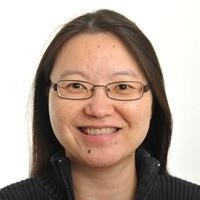
\includegraphics[width=\linewidth]{img/teri.jpg}
                                \centerline{Teri Ngo}
                            \end{minipage}
                            \hspace{0.1cm}
                            \begin{minipage}{0.3\linewidth}
                                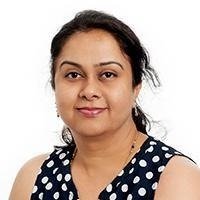
\includegraphics[width=\linewidth]{img/kshama.jpg}
                                \centerline{Kshama Aswath}
                            \end{minipage}
                            \hspace{0.1cm}
                            \begin{minipage}{0.3\linewidth}
                                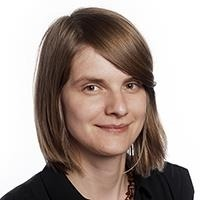
\includegraphics[width=\linewidth]{img/antje.jpg}
                                \centerline{Antje Kazimiers}
                            \end{minipage}
                        \end{addmargin}
                        \begin{addmargin}[1em]{1em}
                            \vspace{1.5cm}
                            \begin{minipage}{0.3\linewidth}
                                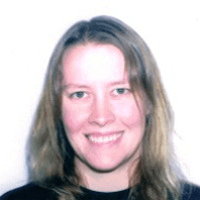
\includegraphics[width=\linewidth]{img/lisa.png}
                                \centerline{Lisa Taylor}
                            \end{minipage}
                            \hspace{0.1cm}
                            \begin{minipage}{0.3\linewidth}
                                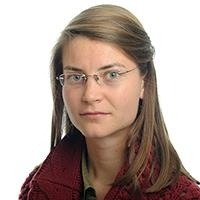
\includegraphics[width=\linewidth]{img/hannah.jpg}
                                \centerline{Hannah Haberkern}
                            \end{minipage}
                            \hspace{0.1cm}
                            \begin{minipage}{0.3\linewidth}
                                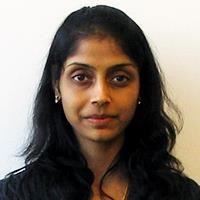
\includegraphics[width=\linewidth]{img/sarada.jpg}
                                \centerline{Sarada Viswanathan}
                            \end{minipage}
                            \begin{addmargin}[.5em]{.5em}
                                \vspace{.75cm}
                                \centerline{and you...?} 
                                \end{addmargin}
                            \end{addmargin}
                    \end{myblock}
                    \vspace{1.25cm}
                    \begin{myblock}{Classes}
                        \begin{addmargin}[1em]{1em}
                            We continue to design and offer courses in a variety of programming languages and topics. Classes offered so far include: 
                        \end{addmargin}
                        \begin{addmargin}[1em]{1em}
                            \begin{figure}
                                \vspace{.5cm}
                                \centering
                                \raisebox{-.5\height}{
\includegraphics[width=0.5\textwidth]{img/pythonlogo.png}}
                                \centering
                                \raisebox{-.5\height}{
\includegraphics[width=0.35\textwidth]{img/R_logo.png}}
                                \vspace{.5cm}
                            \end{figure}
                            \vspace{0.9cm}
                            \begin{figure}
                                \vspace{.5cm}
                                \centering
                                \raisebox{-.5\height}{
\includegraphics[width=0.4\textwidth]{img/latex_logo.png}}
                                \centering
                                \raisebox{-.5\height}{
\includegraphics[width=0.5\textwidth]{img/terminal_image.png}}
                                \vspace{.5cm}
                            \end{figure}
                        \end{addmargin}
                        \vspace{1.6cm}
                        \begin{addmargin}[1em]{1em}
                            All WCC code can be found at \url{github.com/WomensCodingCircle} under open source licenses for member use.
                        \end{addmargin}

                    \end{myblock}\vfill
                    
		}\end{minipage}\end{beamercolorbox}
	\end{column}
  \begin{column}{.33\textwidth}
		\begin{beamercolorbox}[center,wd=\textwidth]{postercolumn}
			\begin{minipage}[T]{.95\textwidth}
				\parbox[t][\columnheight]{\textwidth}{
					\begin{myblock}{About us}
                        \begin{addmargin}[1em]{1em}
                            The WCC meets regularly to discuss any topics related to being a woman in science and programming. We host speakers, teach classes, and explore new technologies together in a supportive environment. We aim to empower women to pursue new programming and technical skills and believe this will make Janelia both a better workplace and a better research institution. 
                        \end{addmargin}
                    \end{myblock}
                    \vspace{1cm}
                    \begin{myblock}{Past Work}
                        \begin{addmargin}[.5em]{.5em}
                            The WCC has undertaken many projects to help our members learn new technologies that might be applicable to their own work, from web applications...
                        \end{addmargin}
                        \begin{addmargin}[1em]{1em}
                            \begin{figure}
                                \vspace{.5cm}
                                \centering
\includegraphics[width=0.59\textwidth]{img/web_app_wcc.png}
                                \vspace{.5cm}
                            \end{figure}
                        \end{addmargin}
                        
                        \begin{addmargin}[1em]{1em}
                            ...to participating in Janelia's first annual Pixy Robot Race
                        \end{addmargin}
                        \begin{addmargin}[1em]{1em}
                            \begin{figure}
                                \vspace{.5cm}
                                \centering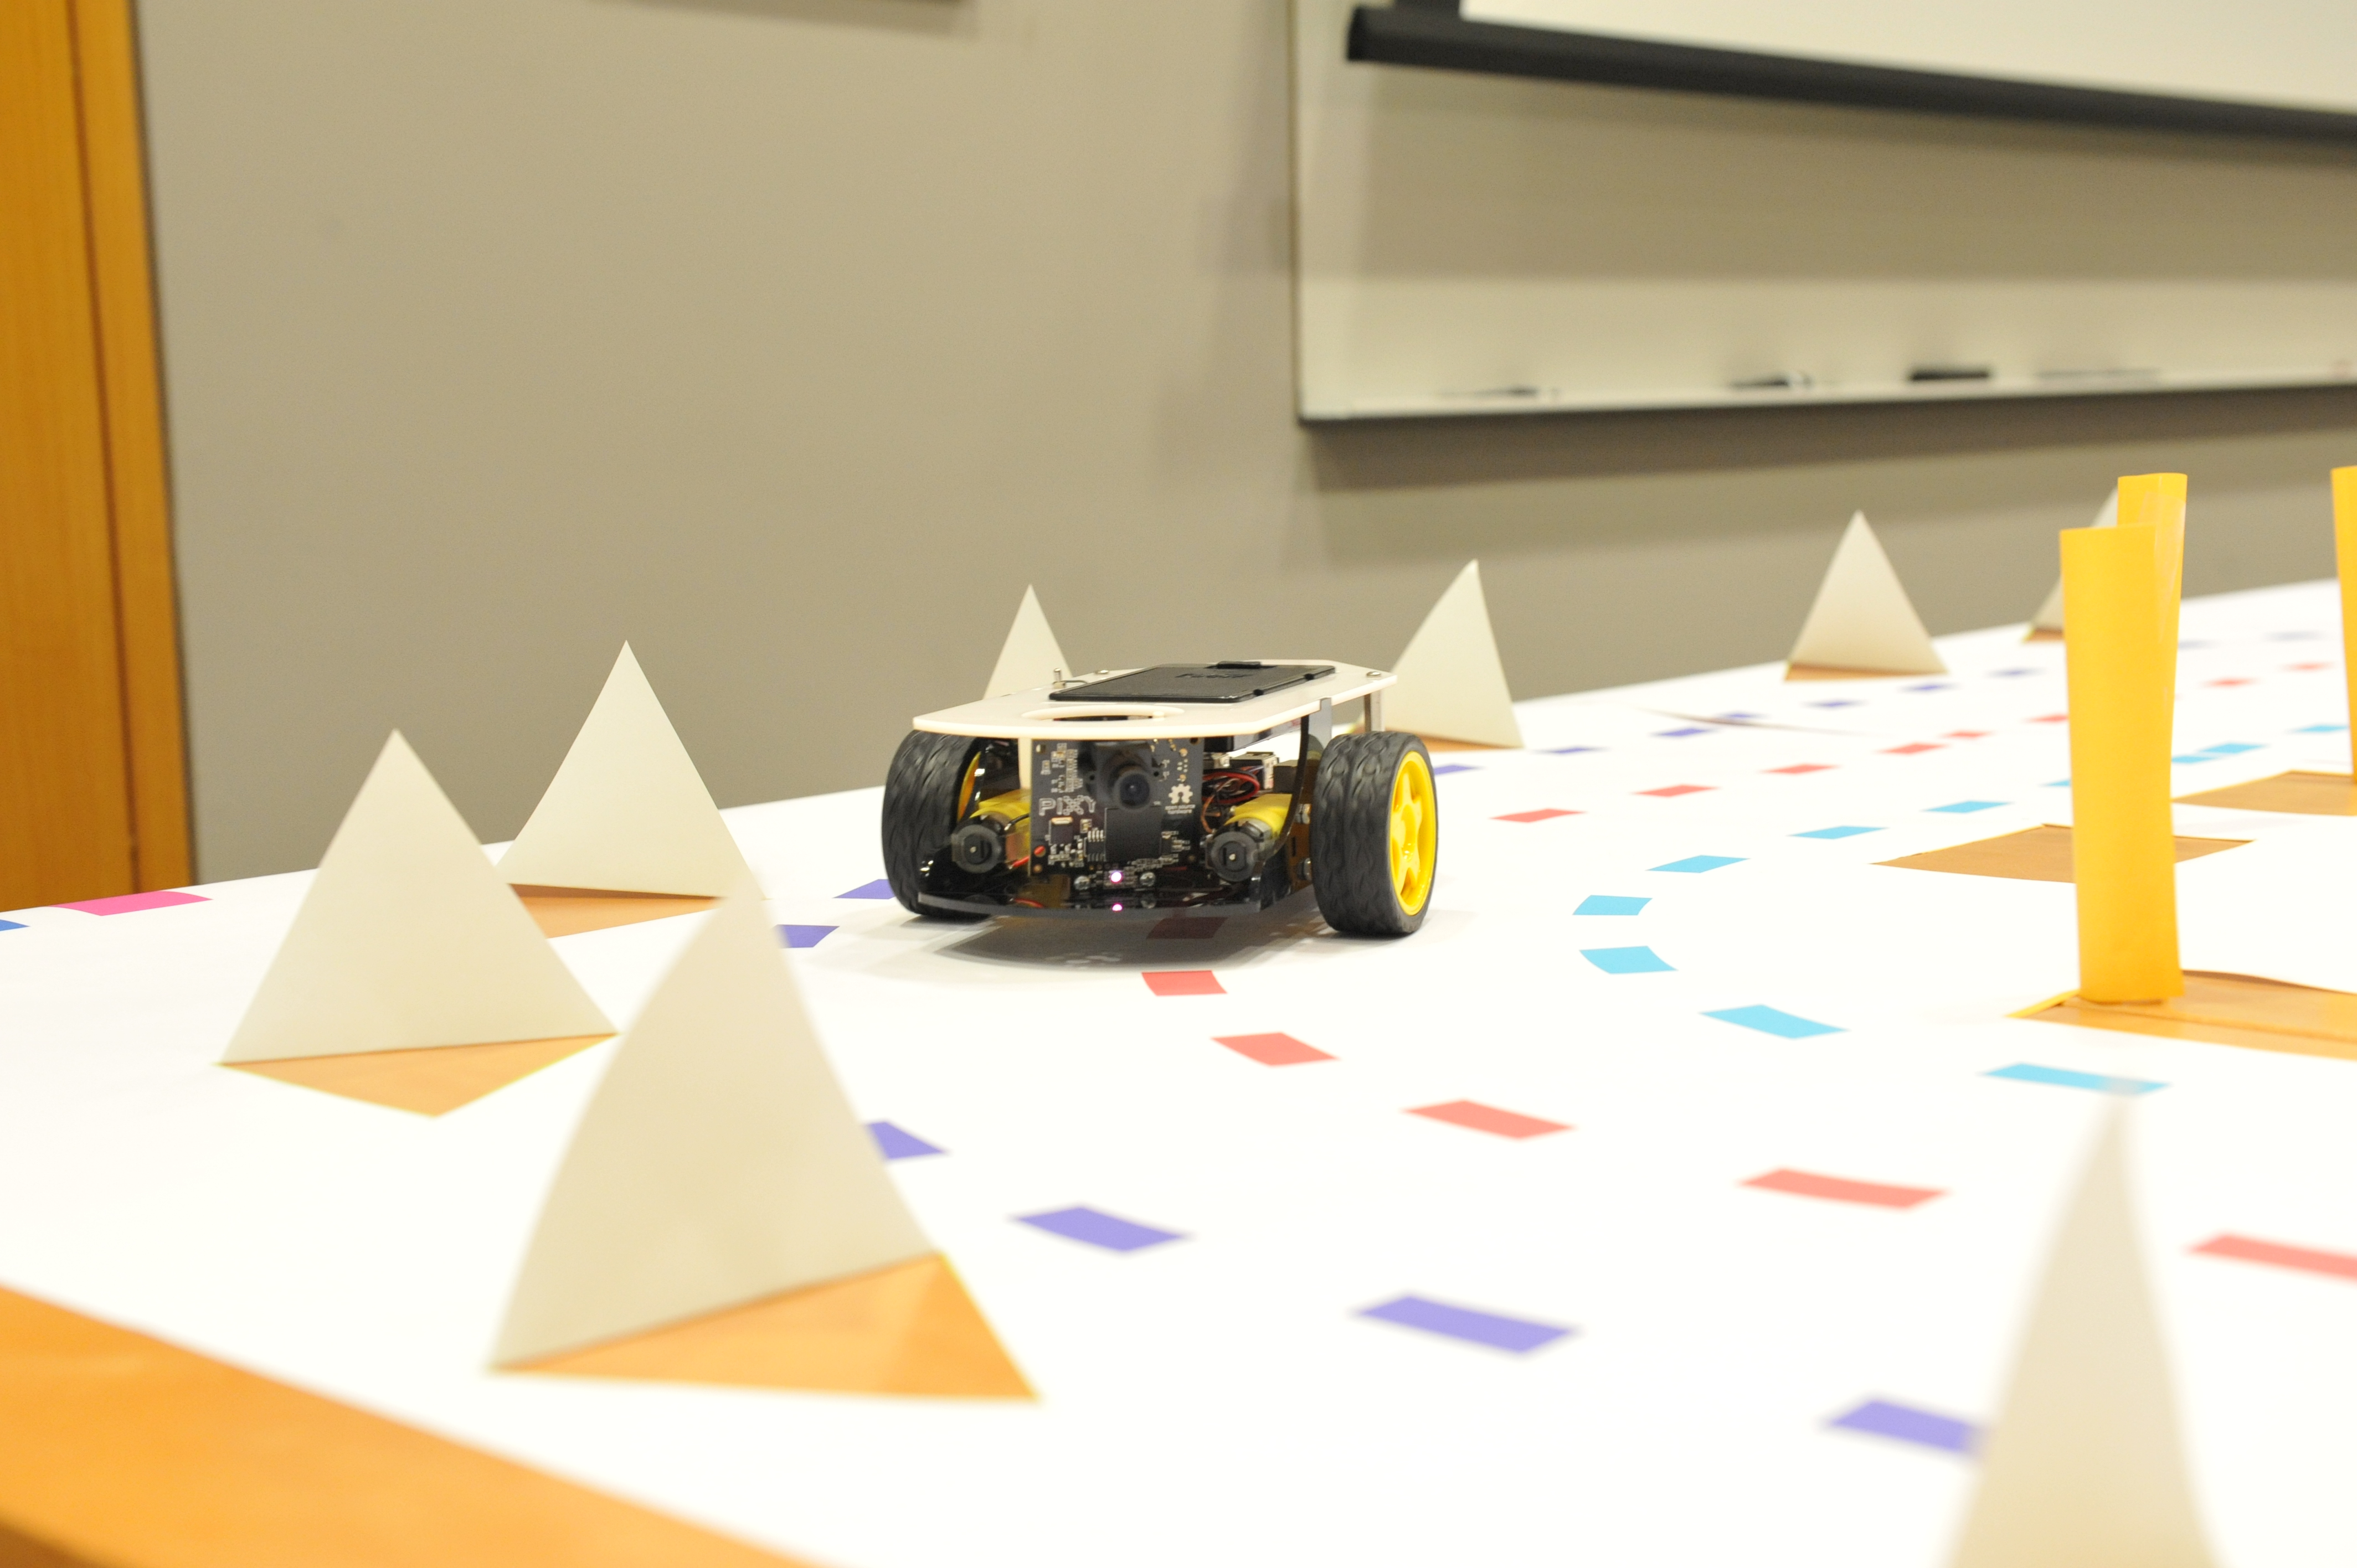
\includegraphics[width=0.59\textwidth]{img/robot.jpg}
                                \vspace{.5cm}
                            \end{figure}
                        \end{addmargin}
                    \end{myblock}
                    \vspace{1cm}
                    \begin{myblock}{Want to join?}
                        \begin{addmargin}[1em]{1em}
                            Our events are open to all women in Janelia, including spouses, children, and anyone else who identifies as a woman. To join the club, please reach out to one of the officers. We will sign you up for our mailing list and Slack channel.
                        \end{addmargin}
                        \vspace{0.6em}
                    \end{myblock}}
		        \end{minipage}\end{beamercolorbox}
  \end{column}
	\begin{column}{.33\textwidth}
		\begin{beamercolorbox}[center,wd=\textwidth]{postercolumn}
			\begin{minipage}[T]{.95\textwidth}
				\parbox[t][\columnheight]{\textwidth}{
					\begin{myblock}{Speakers Series}
            \begin{addmargin}[1em]{1em}
                We invite people in leadership roles in HHMI to talk with our group about their scientific background, why they chose their field, mentors, and role models.
                \vspace{1cm}
            \end{addmargin}
            \begin{addmargin}[1em]{1em}
                \centering
                \begin{minipage}{0.4\linewidth}
                    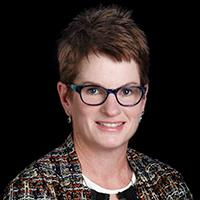
\includegraphics[width=\linewidth]{img/erin.jpg}
                    \centerline{Erin O'Shea, PhD}\newline
                    \centerline{President of HHMI}
                \end{minipage}
                \hspace{0.75cm}
                \begin{minipage}{0.4\linewidth}
                    
\includegraphics[width=\linewidth]{img/kathryn.jpg}
                    \centerline{Kathryn Brown}\newline
                    \centerline{Chief of Communications, HHMI}
                \end{minipage}
            \end{addmargin}
            \vspace{1cm}
            % Kristin / Roian
            \begin{addmargin}[1em]{1em}
                \centering
                \begin{minipage}{0.4\linewidth}
                    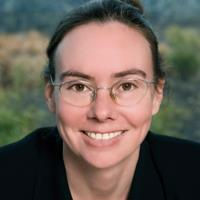
\includegraphics[width=\linewidth]{img/roian.jpg}
                    \centerline{Roian Egnor, PhD}\newline
                    \centerline{Janelia Senior Scientist}
                \end{minipage}
                \hspace{0.75cm}
                \begin{minipage}{0.4\linewidth}
                    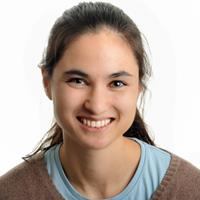
\includegraphics[width=\linewidth]{img/kristin.jpg}
                    \centerline{Kristin Branson, PhD}\newline
                    \centerline{Janelia Senior Group Leader}
                \end{minipage}
            \end{addmargin}
            \vspace{1cm}

            % Jennifer
            \begin{addmargin}[1em]{1em}
                \centering
                \begin{minipage}{0.4\linewidth}
                    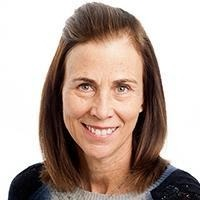
\includegraphics[width=\linewidth]{img/jennifer.png}
                    \centerline{Jennifer Lippincott-Schwartz, PhD}\newline
                    \centerline{Senior Group Leader}
                \end{minipage}
                \hspace{0.75cm}
                \begin{minipage}{0.4\linewidth}
                    
\includegraphics[width=\linewidth]{img/placeholder.png}
                    \centerline{Who?}\newline
                \end{minipage}
            \end{addmargin}
          \end{myblock}\vspace{1.25cm}
          \begin{myblock}{Upcoming events}
                        \begin{addmargin}[1em]{1em}
                            \begin{enumerate}
                                \item Speaker Series with Jan Funke, Nov 1st, 2019, PRISM
                                \item All-hands meeting
                            \end{enumerate}
                        \end{addmargin}
                    \end{myblock}
		}\end{minipage}\end{beamercolorbox}
	\end{column}
\end{columns}
\end{frame}
\end{document}
